\documentclass{beamer}
\usepackage{graphicx}

\title{Deep G-Buffers for stable Global Illumination Approximation}
\author{Ferit Tohidi Far}
\usetheme{Frankfurt}

\begin{document}
	\maketitle

	\begin{frame}
		\frametitle{Content}
		\begin{itemize}
			\item Global illumination
				\begin{itemize}
					\item Pathtracing
					\item Radiosity
				\end{itemize}
			\item Forward rendering
			\item Deferred rendering (with G-Buffers)
			\item Visual effects
				\begin{itemize}
					\item Ambient occlusion
					\item Color bleeding
					\item Soft shadows
					\item Transparency
					\item Reflections
				\end{itemize}
			\item Deferred rendering (with Deep G-Buffers)
		\end{itemize}
	\end{frame}

	\begin{frame}
		\frametitle{Global illumination}
		\begin{itemize}
			\item lights a scene
			\item considers direct and indirect light
			\item causes visual effects that convey realism
		\end{itemize}
	\end{frame}

	\begin{frame}
		\frametitle{Visual effects}
		\begin{center}
			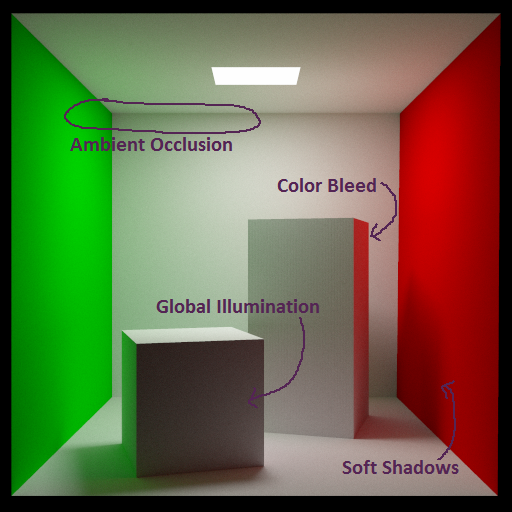
\includegraphics[width=.7\textwidth]{img/visual_effects.png}
		\end{center}
	\end{frame}

	\begin{frame}
		\frametitle{Pathtracing}
		\begin{itemize}
			\item send camera ray through each pixel
			\item trace it back to light source
			\item if light source was hit, the pixel is colored (albedo of object it hit)
			\item else it is black (in shadow)
			\item each pixel is sampled thousands of times, then averaged
		\end{itemize}
	\end{frame}

	\begin{frame}
		\frametitle{Radiosity}
		\begin{itemize}
			\item scene is divided into patches
			\item each patch is a light emitter and receiver
			\item iteratively update emmitance and radiance of each patch
		\end{itemize}
	\end{frame}

	\begin{frame}
		\frametitle{Forward rendering}
		\begin{itemize}
			\item compute lighting and shading in a single pass
			\item inefficient
		\end{itemize}
	\end{frame}

	\begin{frame}
		\frametitle{Deferred rendering (with G-Buffers)}
		\begin{itemize}
			\item collect g-buffers in first pass
			\item compute lighting in second pass
		\end{itemize}
	\end{frame}

	\begin{frame}
		\frametitle{Deferred rendering (with Deep G-Buffers)}
		\begin{itemize}
			\item generate 2-layer deep g-buffer with depth peeling
			\item enforce minimum depth separation
			\item consider second layer for visual effects
		\end{itemize}
	\end{frame}	

	\begin{frame}
		\frametitle{Results}
		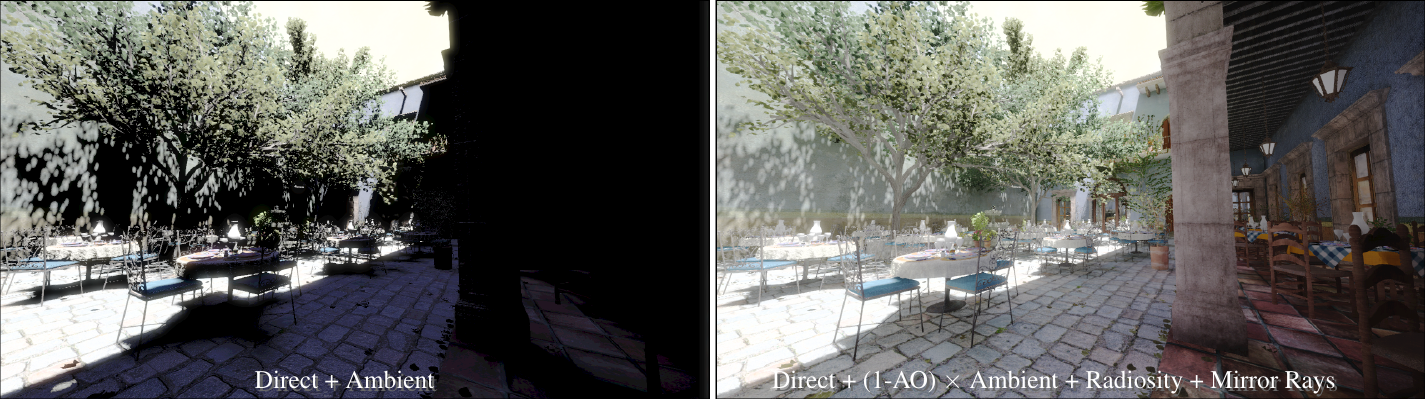
\includegraphics[width=\textwidth]{img/deep_g_buffer_render.png}
		\begin{itemize}
			\item using NVIDIA GeForce 980
			\item image was generated in 10.8ms (92 FPS)
		\end{itemize}
	\end{frame}

\end{document}